\documentclass[conference]{IEEEtran}
\IEEEoverridecommandlockouts

\usepackage{cite}
\usepackage{amsmath,amssymb,amsfonts}
\usepackage{graphicx}
\usepackage{textcomp}
\usepackage{booktabs}
\usepackage{tabularx}
\usepackage{array}
\usepackage{xcolor}
\usepackage{algorithm}
\usepackage{algpseudocode}
\usepackage{tikz}
\usetikzlibrary{arrows.meta,positioning,shapes.geometric,shapes.misc,calc}
\usepackage[hidelinks]{hyperref}

\graphicspath{{./}{figures/}}
\renewcommand{\arraystretch}{1.12}
\newcolumntype{Y}{>{\raggedright\arraybackslash}X}
\setlength{\emergencystretch}{1.5em}
\newcommand{\netSD}{net~$\Sigma D$}
\newcommand{\NetSD}{Net~$\Sigma D$}

\begin{document}

\title{Measuring What a Digital-Twin Validation Gate Buys: Counterfactual Labelling of Every Proposal Across Twin Fidelity}

\author{\IEEEauthorblockN{Nitin Kumar Pandey\textsuperscript{1}, Ayush Raj\textsuperscript{2}, Abhay Mahantesh Zalaki\textsuperscript{3},\\ Guneet Kaur Arora\textsuperscript{4}, Syamasudha Veeragandham\textsuperscript{5}}
\IEEEauthorblockA{\textsuperscript{1,2,3,4,5}School of Computer Science and Engineering, Vellore Institute of Technology,\\
Vellore, Tamil Nadu, India -- 632014\\
Email: \textsuperscript{1}nitinkumar.pandey2023@vitstudent.ac.in, \textsuperscript{2}ayush.raj2023a@vitstudent.ac.in,\\
\textsuperscript{3}abhay.mahantesh2023@vitstudent.ac.in, \textsuperscript{4}guneetkaur.arora2023@vitstudent.ac.in,\\
\textsuperscript{5}syamsudha.v@vit.ac.in\\
\textsuperscript{5}Corresponding author}}

\maketitle

\begin{abstract}
Placing a digital twin between an autonomous controller and a live system, and applying only the actions the twin predicts to be acceptable, is an established safeguard. Its value is usually reported as improvement over an ungated controller, which cannot separate the twin's prediction from the effect of blocking. We present a controller-agnostic measurement method: every proposal, including rejected ones, receives a paired counterfactual label from the real simulator, and every twin-gated arm is compared with a reject-all gate that makes no prediction. We apply it to a deterministic edge-network simulator with a twin degraded along five fidelity axes, using 150 paired seeds, 6 fidelity levels, a rule-based and a scripted controller, and exact paired tests with Holm correction. Unvalidated action is harmful, and a low-fidelity twin is worse than no gate. The locally measured net benefit of the approved set crosses zero near fidelity 0.549 for the scripted controller, and this crossing survives holding the twin's queueing model constant. At the episode level the twin beats reject-all only for the rule controller at fidelity 1.0 and 0.8, by about 1.9\% of baseline violations, carried by 14.7\% of seeds; the fidelity-1.0 result survives Bonferroni correction. The ceiling on any gate's gain is the benefit that reject-all discards, which is small for both controllers. Classifier quality is best read where the harm threshold equals the gate tolerance, which is not the best operating point. Local counterfactuals do not compose into episode effects. A 30-seed live-model study is reported descriptively only. Gate evaluations should report a reject-all control, per-seed distributions and the benefit actually available to the gate.
\end{abstract}

\begin{IEEEkeywords}
Digital twin, validation gate, counterfactual evaluation, twin fidelity, edge networks, autonomous remediation, LLM agents, reject-all control
\end{IEEEkeywords}

\section{Introduction}

\textbf{Background: autonomous operation of networked services.} Operating edge and IoT networks under faults such as saturated nodes, crashed devices, degraded links, memory leaks, and traffic surges requires remediation decisions faster than human operators can make them. These decisions are increasingly delegated to automated controllers and, more recently, to agents driven by large language models (LLMs). Benchmarks now evaluate such agents on microservice remediation~\cite{microremed}, network troubleshooting~\cite{nika}, and stateful network configuration~\cite{netagentbench}, which shows that autonomous operation is an active research target rather than a distant prospect.

\textbf{Digital twins as a pre-actuation safeguard.} A wrong action applied to a live network can cause lasting damage, so a recurring design places a digital twin between the decision maker and the network. The proposed change is first executed on the twin, and only changes predicted to be acceptable are applied. Aether coordinates network-operations agents with a network digital twin to validate configuration changes on an ISP laboratory replica~\cite{aether}, and recent process-plant work lets an LLM agent propose actions that are validated in simulation and re-prompted on failure~\cite{processplant}, and infrastructure-orchestration work treats the twin as a mandatory gate between an optimisation agent and the execution layer~\cite{twingatedorch}. The twin-gated pattern is therefore established; what is less established is how to measure what the twin contributes.

\textbf{Lineage in safety-critical control.} The idea of checking an advanced controller's output against a model before actuation predates LLMs. The Simplex architecture separates a high-performance controller from a simple verified safety controller that takes over before failure~\cite{bbsimplex}. Predictive safety filters forward-simulate a proposed input and minimally modify it when it cannot be certified~\cite{wabersich}, and model predictive shielding uses forward simulation to decide whether a learned policy may act or must hand control to a backup policy~\cite{dmps}. Finite-horizon prediction, terminal conditions, and robustness to model error are central design concerns in model predictive control~\cite{mpcreview}. Our gate is a deliberately simple member of this family.

\textbf{Motivation: outcome improvement does not measure prediction.} Evaluating a twin gate is harder than building one. Real networks cannot be replayed, so the true consequence of a \emph{rejected} change is rarely observed, and evaluations tend to report outcome improvement over an ungated agent. That comparison conflates two sources of benefit: the gate's ability to tell good actions from bad ones, and the simple fact that it blocks something. If most of an agent's proposals are harmful, a gate that blocks everything looks excellent while predicting nothing. NetInjectBench makes this concrete for tool-using network agents by showing that a static allowlist reduces unsafe actions but destroys the usefulness of approved changes~\cite{netinjectbench}.

\textbf{Motivation: safety must be reported with utility.} Security evaluations of agents have converged on reporting utility and attack success together, because either number alone can be optimised trivially. AgentDojo reports utility, utility under attack, and attack success side by side and cautions against reducing them to a single leaderboard~\cite{agentdojo}. The analogous requirement for twin gates is that harm prevented must be reported together with benefit preserved, and both must be compared with a no-prediction control.

\textbf{Motivation: twins are never exact.} Any deployed twin differs from the system it models through observation noise, stale state, drifting parameters, forecast error, and simplified dynamics. Monotone gains with fidelity should not be assumed: in additive manufacturing, lower-fidelity twins can detect failures comparably to higher-fidelity ones~\cite{fidelityam}. Model-based reinforcement learning likewise studies how prediction length trades usefulness against compounding model bias~\cite{mbrlsurvey}. Fidelity is rarely varied systematically in agentic network settings, which motivates a controllable-fidelity twin.

\textbf{Motivation: faults are only partially observable.} A controller sees symptoms, not causes, and a twin rolled forward from the current state cannot know which faults will arrive in the future. Whether a fault can be inferred from observed behaviour is a question of diagnosability that is distinct from state observability~\cite{robustdiag}, and planning under partial observability typically relies on sampling hidden states through a black-box simulator~\cite{pomdpsurvey}. We make this limitation explicit by rolling the twin forward \emph{fault-blind} and comparing it with a gate that can see the schedule.

\textbf{Motivation: operational repair semantics matter.} Real repair actions have costs and interact. Production orchestrators implement reconciling control loops that drive observed state toward desired state~\cite{k8scontroller}, autoscalers use tolerances and stabilisation windows to avoid oscillation~\cite{k8shpa}, and studies of production incidents show how load shifted onto surviving replicas can trigger self-sustaining cascading overload~\cite{metastable}. A testbed that treats restarts and migrations as free would overstate the value of acting, so our simulator charges explicit downtime and drops.

\textbf{Motivation: bounded agents need bounded evaluation.} Agent loops are bounded by step or tool budgets, and behaviour at the bound affects outcomes. Budget-aware tool use shows that exposing the remaining budget changes how agents scale~\cite{budgetaware}, and graph-based agent frameworks raise explicit errors when recursion limits are reached~\cite{langgraph}. Our controllers operate under a bounded retry budget with a no-op fallback, so the gate's rejection behaviour and the controller's retry behaviour must be analysed together.

\textbf{Scope: a measurement instrument, not a new safety guarantee.} Using common random numbers to compare alternatives in simulation is standard~\cite{stochsim}, and it has recently been applied to rollout-based planning, where the continuation policy affects the variance of relative utilities~\cite{yadav}. Action-level safety labels and shields have been formalised with explicit false positives and negatives~\cite{rulebasedshield}, and safe and constrained reinforcement learning has been surveyed extensively~\cite{saferlsurvey}. We do not claim that twin-gated validation, paired simulation, or shielding is new. The contribution is a testbed and protocol that isolate what the twin's \emph{prediction} adds, run on a synthetic simulator whose limits are stated in Section~\ref{sec:limits}.

\textbf{Contributions.} Building on the twin-gate architecture of prior work~\cite{aether,processplant,twingatedorch}, the paper makes four contributions. (i) A controller-agnostic measurement method that labels every proposal, including rejected ones, with a paired counterfactual harm delta from the real system and scores every twin-gated arm against a reject-all gate on the same seeds. (ii) A characterisation of how the twin's value depends on fidelity along five controllable axes, including a control that holds the twin's queueing model constant. (iii) Results at 150 paired seeds for two proposers, with a live-model study as one further, descriptive proposer. (iv) A methodological finding that local counterfactuals do not compose into episode effects, with its mechanism.

\subsection{Research Objectives}

\begin{enumerate}
  \renewcommand{\labelenumi}{\textbf{RO\arabic{enumi}.}}
  \item To define a controller-agnostic protocol that labels every proposal, including rejected ones, with a paired counterfactual harm delta and scores a twin gate against a reject-all control, both as a harm classifier and by closed-loop SLO violations.
  \item To characterise how the value of the gate depends on twin fidelity along five controllable axes, and to test whether the observed fidelity crossover is attributable to fidelity rather than to a discrete change in the twin's queueing model.
  \item To determine with exact paired statistics at 150 seeds whether a twin gate improves episode outcomes beyond no-prediction controls, and to bound the gain any gate can achieve by the benefit reject-all discards.
  \item To test whether local counterfactual metrics compose into episode-level effects, and to describe a live language-model proposer with the same instrument.
\end{enumerate}

\section{Related Work}

\textbf{Digital twins for network change validation.} Aether coordinates five network-operations agents with a network digital twin to validate configuration changes on a 25-router ISP laboratory replica~\cite{aether}. It reports 94\% error detection with 0.64 precision on synthetic scenarios and 100\% detection on two past incidents, while final deployment approval remains with a human. It does not sweep twin fidelity or report a reject-all control. Our work is complementary: a far simpler network, but a protocol that isolates prediction from blocking.

\textbf{LLM agents with simulation-in-the-loop fault handling.} The process-plant study of~\cite{processplant} is the closest propose--simulate--validate--reprompt architecture. It reports correct, incorrect, and missed actions and reprompt counts across models and input representations for a clogging scenario. Its agent has access to state and fault type, and after retries are exhausted it forces the action. Our controllers see symptoms only, and our fallback after rejection is a no-op, which changes what a rejection costs.

\textbf{Remediation benchmarks for services.} MicroRemed benchmarks LLMs that generate remediation playbooks for microservice failures and evaluates recovery~\cite{microremed}. SLBench evaluates skill-following and mitigation behaviour and reports a reduction in violations on a selected set of previously violating cases~\cite{slbench}. These benchmarks measure the proposer; neither isolates the contribution of a model-based validation gate.

\textbf{Network troubleshooting and configuration benchmarks.} NIKA provides an arena for benchmarking agents on realistic network diagnosis and localisation~\cite{nika}, and NetAgentBench evaluates stateful, multi-turn network configuration~\cite{netagentbench}. They supply richer network semantics than our simulator but no counterfactual label for rejected actions, which is the quantity our protocol is built around.

\textbf{Safety versus utility for tool-using agents.} NetInjectBench reports unsafe tool-action rates for network agents under indirect prompt injection and shows that a static allowlist achieves safety at the cost of approved-change usefulness~\cite{netinjectbench}. AgentDojo reports utility and attack success jointly~\cite{agentdojo}. Our reject-all ablation applies the same principle to a closed-loop network setting: a gate that never approves anything is the baseline that prediction must beat.

\textbf{Predictive safety filters and shielding.} Simplex~\cite{bbsimplex}, predictive safety filters~\cite{wabersich}, and model predictive shielding~\cite{dmps} forward-simulate a proposed action and fall back to a backup policy. Data-driven safety filters extend these ideas to uncertain and stochastic dynamics~\cite{ddsafety}. These methods provide recoverability guarantees under model assumptions; our gate provides none. It approves an action if predicted violations over a finite horizon are no worse than those of a no-op.

\textbf{Shields and safe reinforcement learning.} Rule-based shields define ground-truth safety labels on state--action pairs and discuss false positives and negatives of a binary shield~\cite{rulebasedshield}. A recent survey maps safe and constrained reinforcement learning across single- and multi-agent settings~\cite{saferlsurvey}. We borrow the classifier view of a shield but add closed-loop episode outcomes and no-prediction controls, since classifier accuracy alone does not establish operational value.

\textbf{Model fidelity and decision-aware modelling.} Su \emph{et al.} vary six digital-twin attributes for material-extrusion failure detection and find that lower-fidelity twins can perform comparably~\cite{fidelityam}. Model-based reinforcement learning studies the tradeoff between rollout length and compounding model bias~\cite{mbrlsurvey}, and value-gradient weighted model learning weights model error by its effect on decisions~\cite{vagram}. Both lines suggest that the relevant question is not how accurate a twin is but whether its errors change decisions, which our fidelity sweep and composition analysis test directly.

\textbf{Common random numbers and paired simulation.} Common random numbers reduce the variance of differences between simulated alternatives~\cite{stochsim}. Yadav \emph{et al.} use them for simulation-based planning with rollouts and show that the continuation policy affects relative-utility variance~\cite{yadav}. Our paired action/no-op forks implement this established technique; they are not a new causal method, and our labels inherit the no-op continuation assumption.

\textbf{Diagnosability and planning under partial observability.} Diagnosability asks whether observed behaviour can establish that a fault occurred~\cite{robustdiag}, a question also studied for event patterns in labelled time Petri nets~\cite{petridiag}. Online POMDP planners such as POMCP plan with a black-box simulator by sampling hidden states from a belief~\cite{pomdpsurvey}. Our fault-blind twin sits at the simplest end of this space: it assumes current faults persist and future faults do not occur, and a schedule-aware gate quantifies the cost of that assumption.

\textbf{Operational control loops and observability practice.} Kubernetes controllers reconcile observed and desired state~\cite{k8scontroller}, and the HorizontalPodAutoscaler uses metric ratios, tolerances, and stabilisation windows~\cite{k8shpa}. Surveys of anomaly detection and root-cause analysis for microservice applications separate observed symptoms from root causes~\cite{rcasurvey}, and studies of production incidents characterise cascading, self-sustaining overload~\cite{metastable}. These practices inform our action costs and SLO definitions, but production systems rarely log counterfactual outcomes of rejected changes, which is why a deterministic testbed is useful.

\textbf{Twin-gated orchestration.} Recent infrastructure-orchestration work describes a digital twin as a mandatory validation gate between an optimisation agent and the execution layer, with failed candidates returned to the agent for re-optimisation~\cite{twingatedorch}. This is the gate-plus-retry loop we adopt; like the other twin-gate studies, it does not score rejected candidates against a counterfactual or compare with a reject-all gate.

\begin{table*}[t]
\centering
\caption{Representative prior works and their relationship to this work.}
\label{tab:related}
\small
\begin{tabularx}{\textwidth}{@{}p{2.6cm}p{2.5cm}YYY@{}}
\toprule
Work & Domain & Validation / safety mechanism & Evaluation controls reported & Relationship to this work \\
\midrule
Aether~\cite{aether} & ISP network change validation & Network digital twin with agents; human approval & Detection rate, precision on synthetic and historical incidents & Same pattern; we add fidelity sweep and reject-all control \\
Process plant~\cite{processplant} & Industrial process control & Simulation validation with LLM re-prompting & Correct / incorrect / missed actions, reprompts & Closest loop; our agents see symptoms only and fall back to no-op \\
MicroRemed~\cite{microremed} & Microservices & None (proposer benchmark) & Recovery success & Measures proposer; we measure the gate \\
NIKA~\cite{nika}, NetAgentBench~\cite{netagentbench} & Network troubleshooting, configuration & None (proposer benchmark) & Diagnosis and configuration correctness & Richer networks; no counterfactual labels \\
NetInjectBench~\cite{netinjectbench} & Network agent security & Allowlist and defences & Unsafe-action rate with utility & Same safety--utility principle, open-loop \\
Predictive safety filter~\cite{wabersich}, MPS~\cite{dmps} & Continuous control & Forward simulation with backup policy & Constraint satisfaction guarantees & Theoretical lineage; our gate gives no guarantee \\
Rule-based shield~\cite{rulebasedshield} & Reinforcement learning & Learned action-level shield & False positives / negatives & Classifier view we adopt and extend \\
Su \emph{et al.}~\cite{fidelityam} & Additive manufacturing & Digital-twin failure detection & Detection across fidelity levels & Fidelity need not be monotone; we test for gating \\
Orchestration twin gate~\cite{twingatedorch} & Compute-infrastructure orchestration & Twin as mandatory gate with re-optimisation & Constraint satisfaction of candidates & Same gate-plus-retry loop; no counterfactual or reject-all control \\
\textbf{This work} & Edge / IoT network (simulated) & Fault-blind twin gate, 5 fidelity axes, 6 levels & Counterfactual label for every proposal; reject-all, random and schedule-aware controls; exact tests at 150 seeds & -- \\
\bottomrule
\end{tabularx}
\end{table*}

\subsection*{Gaps}

\begin{enumerate}
  \renewcommand{\labelenumi}{\textbf{G\arabic{enumi}.}}
  \item Twin-gated validation is usually evaluated against an ungated agent, without a reject-all or random-gating control, so improvement cannot be attributed to prediction.
  \item Twin fidelity is rarely varied along independent, controllable axes, and discrete changes in the twin's model are rarely separated from continuous degradation.
  \item The consequences of rejected actions are seldom labelled, so gates are not scored as classifiers on the same examples on which episode outcomes are measured.
  \item Headline improvements are seldom accompanied by per-seed distributions, exact tests, multiplicity correction, or the amount of benefit a gate could possibly preserve.
\end{enumerate}

\subsection*{Problem Statement}

Given an autonomous controller that proposes repair actions for a faulty edge network and a digital-twin gate that approves or rejects each proposal, determine whether the gate's \emph{predictions} improve closed-loop SLO outcomes beyond what blocking alone achieves; quantify how this depends on twin fidelity and on the controller's candidate actions; and do so with labels for every proposal and statistics that are valid for small, zero-inflated paired samples.

\section{Materials and Methods}

\subsection{Dataset}

No external dataset is used. All data are generated by the simulator and are reproducible from a seed. Each seed fixes the Poisson workload, the fault schedule (3 faults per episode, start ticks 20--260, durations 20--80 ticks, so some faults start after the 120-tick episode ends), and all random streams. Every proposal record carries the controller, gate, tick, retry index, action, twin prediction, verdict, whether it was applied, and its counterfactual harm delta. Table~\ref{tab:dataset} summarises the corpus.

\begin{table}[t]
\centering
\caption{Generated experimental corpus.}
\label{tab:dataset}
\footnotesize
\begin{tabular}{@{}p{0.5\columnwidth}p{0.42\columnwidth}@{}}
\toprule
Item & Value \\
\midrule
Topology & 1 gateway, 4 edge servers, 12 IoT devices; 6 services \\
Seeds (contiguous) & 150 \\
Fidelity levels & 6 (0.0--1.0) \\
Queueing conditions & 2 \\
Arms per controller & 10 (plus null reference) \\
Episodes in the fidelity sweep & 6{,}300 (3{,}150 per condition) \\
Twin@1.0 labelled candidates (rule / scripted) & 159 / 1{,}167 \\
Live-model study & 30 seeds $\times$ 4 arms \\
\bottomrule
\end{tabular}
\end{table}

\textbf{Data split.} There is no training, so there is no train/test split. The design is paired: every arm runs on identical seeds, fault schedules and controller code, and only the gate differs. All 150 seeds were fixed before any outcome was observed.

\subsection{System Architecture}

Figure~\ref{fig:arch} shows the control loop. Four design principles govern it: (i) the simulator is the ground truth and is deterministic given a seed, which makes counterfactual evaluation possible; (ii) the twin is never assumed to be perfect; (iii) all controllers share one interface, so experimental arms differ only by configuration; and (iv) actions come from a closed schema, so free-form commands never reach the simulator.

\begin{figure*}[t]
\centering
\resizebox{0.8\textwidth}{!}{%
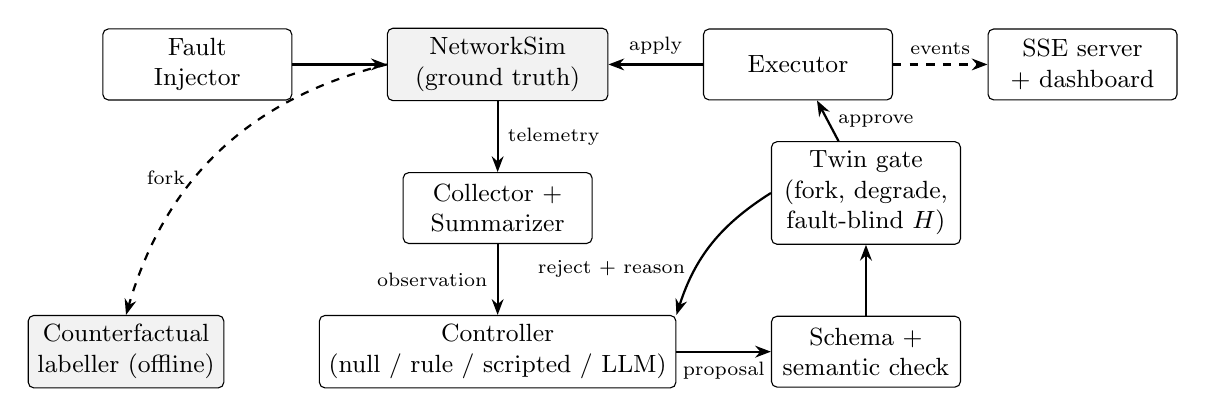
\begin{tikzpicture}[
  box/.style={draw, rounded corners=2pt, align=center, minimum height=0.9cm, minimum width=2.4cm, font=\small},
  arr/.style={-{Stealth[length=2mm]}, thick},
  dasharrow/.style={-{Stealth[length=2mm]}, thick, dashed}
]
\node[box] (fi) {Fault\\Injector};
\node[box, right=1.2cm of fi, minimum width=2.8cm, fill=gray!10] (sim) {NetworkSim\\(ground truth)};
\node[box, right=1.2cm of sim] (ex) {Executor};
\node[box, below=0.9cm of sim] (tel) {Collector +\\Summarizer};
\node[box, below=0.9cm of tel] (ag) {Controller\\(null / rule / scripted / LLM)};
\node[box, right=1.2cm of ag] (val) {Schema +\\semantic check};
\node[box, above=0.9cm of val] (tw) {Twin gate\\(fork, degrade,\\fault-blind $H$)};
\node[box, left=1.2cm of ag, fill=gray!10] (cf) {Counterfactual\\labeller (offline)};
\node[box, right=1.2cm of ex] (sse) {SSE server\\+ dashboard};
\draw[arr] (fi) -- (sim);
\draw[arr] (ex) -- node[above, font=\scriptsize]{apply} (sim);
\draw[arr] (sim) -- node[right, font=\scriptsize]{telemetry} (tel);
\draw[arr] (tel) -- node[left, font=\scriptsize]{observation} (ag);
\draw[arr] (ag) -- node[below, font=\scriptsize]{proposal} (val);
\draw[arr] (val) -- (tw);
\draw[arr] (tw) -- node[right, font=\scriptsize]{approve} (ex);
\draw[arr] (tw.west) to[bend right=20] node[left, font=\scriptsize, pos=0.7]{reject + reason} (ag.north east);
\draw[dasharrow] (sim.west) to[bend right=30] node[left, font=\scriptsize, pos=0.6]{fork} (cf.north);
\draw[dasharrow] (ex.east) -- node[above, font=\scriptsize]{events} (sse.west);
\end{tikzpicture}}
\caption{Twin-in-the-Loop architecture. The twin forks the live simulator, degrades the copy according to the fidelity setting, and rolls it forward without the fault schedule. An offline labeller forks the real simulator \emph{with} the schedule to score every proposal; it never influences the live episode.}
\label{fig:arch}
\end{figure*}

\textbf{Network simulator.} The simulator is discrete-time. Each tick applies scheduled fault events, generates Poisson arrivals, routes requests over links, processes service queues with exponential service times and bounded queues with overflow drops, updates utilisation, and emits a metrics record. A service's SLO requires p95 latency $\le 600$\,ms and availability $\ge 99\%$, with an at-risk band from $0.85 \times 600 = 510$\,ms. A tick in which a service completes no requests is non-compliant. The method \texttt{fork()} deep-copies the state, including random-number streams, so a branch replays exactly the exogenous randomness of its parent. Per-service accounting satisfies
\begin{equation}
O_{t} + A_t = C_t + D_t + O_{t+1},
\label{eq:conservation}
\end{equation}
where $O$ is outstanding requests, $A$ arrivals, $C$ completions, and $D$ drops, including requests lost to restart or migration.

\textbf{Fault model.} Six fault types are injectable: \texttt{node\_cpu\_saturation}, \texttt{node\_crash}, \texttt{link\_degradation}, \texttt{link\_failure}, \texttt{service\_memory\_leak}, and \texttt{traffic\_surge}. Each has a target, start tick, duration, and magnitude. Active faults compose: CPU reservations add (capped at 98\% of capacity), link losses add (capped at 1), latency and arrival multipliers multiply, and \emph{down} overrides \emph{degraded}. When a fault expires, only its own contribution is removed. When aggregate memory exceeds host capacity, every request on that host fails until the pressure is relieved. By default, node faults target edge servers only; a \texttt{gateway\_faultable} flag adds the gateway to the node-fault target pool.

\textbf{Action space and validation.} Controllers choose one of six actions: \texttt{migrate\_service}, \texttt{restart\_service}, \texttt{scale\_service}, \texttt{reroute\_traffic}, \texttt{throttle\_service}, and \texttt{no\_op}. Actions carry real costs: a restart makes the service unavailable for three processing ticks, and migrating a five-unit-memory service takes ten. A proposal must pass three layers: (1) a schema layer that rejects unknown types and missing, extra, or mistyped fields; (2) a semantic layer that checks entity existence, replica caps, memory capacity, finite positive rate limits, pending-action conflicts, and route validity; and (3) the twin gate.

\textbf{Controllers.} \emph{Null} always emits \texttt{no\_op}. \emph{Rule} is a threshold controller that, for example, migrates a service off an edge node whose utilisation stays above 90\% while the service is in violation, restarts a service under memory pressure, and scales services in p95 violation when host capacity allows. \emph{Scripted} is a deterministic aggressive scale-or-hold policy that stands in for an aggressive proposer and makes no model calls. An \emph{LLM agent} built on LangGraph, with telemetry tools, a bounded tool-use loop, response caching and a hard budget guard, is used as a further proposer in a descriptive study.

\subsection{Controllable-Fidelity Twin Gate}

At a decision tick $t$ with proposal $a$, the gate forks the live simulator, degrades the fork, and rolls two branches forward for $H$ ticks, one with $a$ applied and one with \texttt{no\_op}. Both run \emph{fault-blind}: faults active at $t$ persist, but scheduled future faults are hidden. Let $\hat{V}_H(a)$ be the predicted violation-ticks. The gate approves if and only if
\begin{equation}
\hat{V}_H(a) - \hat{V}_H(\texttt{no\_op}) \le \tau ,
\label{eq:gate}
\end{equation}
with tolerance $\tau = 0$. A rejection returns a reason to the controller, which may retry up to a cap of two; the fallback is \texttt{no\_op}.

The twin is degraded along five axes. A scalar fidelity $f \in [0,1]$ with $d = 1 - f$ maps onto them (Table~\ref{tab:fidelity}). At $f = 1$ every axis is off and the twin is an exact fork, so it differs from reality only in not seeing the fault schedule. Fidelity noise is drawn from a dedicated seed stream, so changing $f$ never perturbs the real trajectory.

\begin{table}[t]
\centering
\caption{Twin degradation axes and scalar mapping ($d = 1-f$).}
\label{tab:fidelity}
\footnotesize
\setlength{\tabcolsep}{3pt}
\begin{tabular}{@{}p{2.1cm}p{3.5cm}l@{}}
\toprule
Axis & What it degrades & Value \\
\midrule
Observation noise & start-state degradation read & $\sigma = 0.30d$ \\
Staleness & degradation scaled toward baseline & $\mathrm{round}(12d)$ ticks \\
Parameter drift & CPU capacity and CPU demand & $\pm 0.30d$ \\
Forecast error & per-service arrival rates & $\pm 0.40d$ \\
Queueing simplification & exponential $\to$ deterministic service & on if $f<0.5$ \\
\bottomrule
\end{tabular}
\end{table}

\subsection{Flowchart and Algorithm}

Figure~\ref{fig:flow} shows one decision, and Algorithm~\ref{alg:episode} gives the episode loop with offline labelling.

\begin{figure}[t]
\centering
\resizebox{\columnwidth}{!}{%
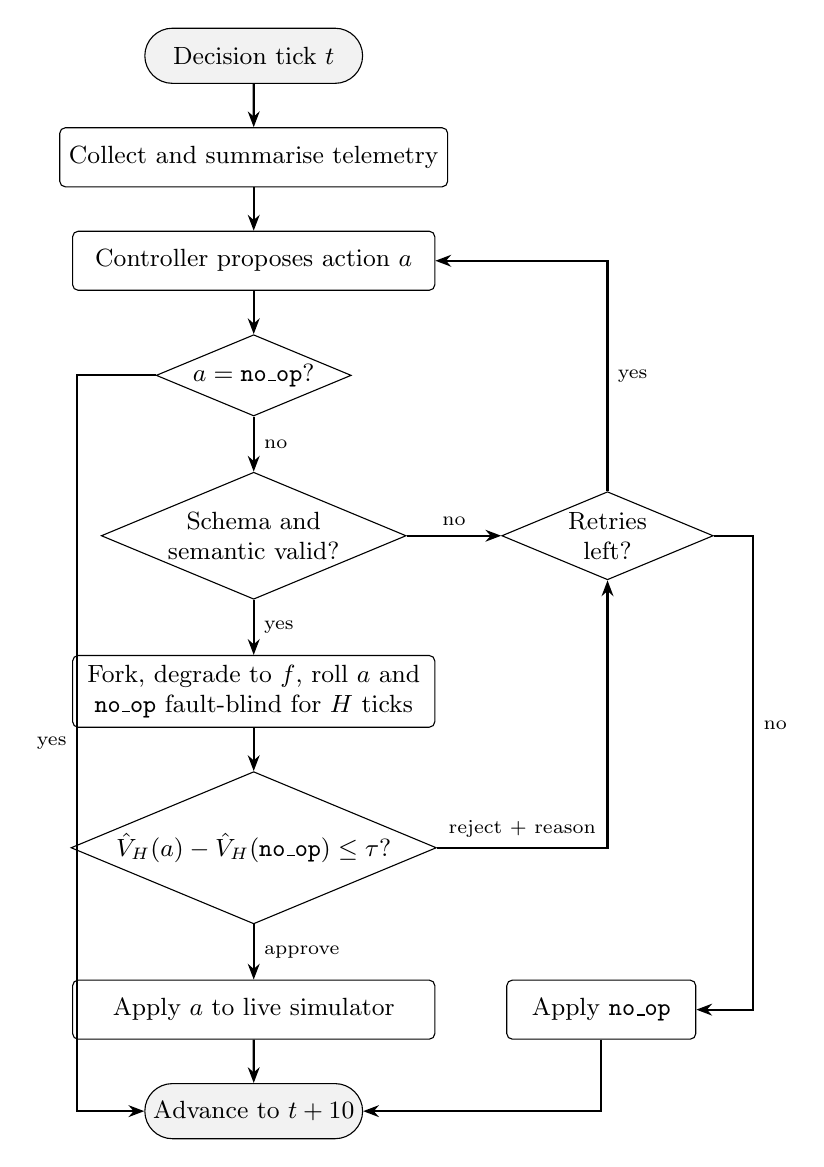
\begin{tikzpicture}[
  node distance=0.55cm,
  proc/.style={draw, rectangle, rounded corners=2pt, align=center, minimum width=4.6cm, minimum height=0.75cm, font=\small},
  dec/.style={draw, diamond, aspect=2.4, align=center, inner sep=1pt, font=\small},
  term/.style={draw, rounded rectangle, align=center, minimum width=3cm, minimum height=0.7cm, font=\small, fill=gray!10},
  arr/.style={-{Stealth[length=2mm]}, thick}
]
\node[term] (s) {Decision tick $t$};
\node[proc, below=of s] (obs) {Collect and summarise telemetry};
\node[proc, below=of obs] (prop) {Controller proposes action $a$};
\node[dec, below=of prop] (noop) {$a = \texttt{no\_op}$?};
\node[dec, below=0.7cm of noop] (valid) {Schema and\\semantic valid?};
\node[proc, below=0.7cm of valid] (twin) {Fork, degrade to $f$, roll $a$ and\\\texttt{no\_op} fault-blind for $H$ ticks};
\node[dec, below=of twin] (gate) {$\hat{V}_H(a) - \hat{V}_H(\texttt{no\_op}) \le \tau$?};
\node[proc, below=0.7cm of gate] (apply) {Apply $a$ to live simulator};
\node[dec, right=1.2cm of valid] (retry) {Retries\\left?};
\node[proc, right=0.9cm of apply, minimum width=2.4cm] (hold) {Apply \texttt{no\_op}};
\node[term, below=of apply] (e) {Advance to $t+10$};
\draw[arr] (s) -- (obs);
\draw[arr] (obs) -- (prop);
\draw[arr] (prop) -- (noop);
\draw[arr] (noop) -- node[right, font=\scriptsize]{no} (valid);
\draw[arr] (valid) -- node[right, font=\scriptsize]{yes} (twin);
\draw[arr] (twin) -- (gate);
\draw[arr] (gate) -- node[right, font=\scriptsize]{approve} (apply);
\draw[arr] (apply) -- (e);
\draw[arr] (valid.east) -- node[above, font=\scriptsize]{no} (retry.west);
\draw[arr] (gate.east) -| node[pos=0.25, above, font=\scriptsize]{reject + reason} (retry.south);
\draw[arr] (retry.north) |- node[pos=0.25, right, font=\scriptsize]{yes} (prop.east);
\draw[arr] (retry.east) -- ++(0.5,0) |- node[pos=0.2, right, font=\scriptsize]{no} (hold.east);
\draw[arr] (noop.west) -- ++(-1.0,0) |- node[pos=0.25, left, font=\scriptsize]{yes} (e.west);
\draw[arr] (hold.south) |- (e.east);
\end{tikzpicture}}
\caption{Flowchart of one gated decision. Rejected or invalid proposals return a reason to the controller, which may retry within its budget; otherwise the system holds.}
\label{fig:flow}
\end{figure}

\begin{algorithm}[t]
\caption{Gated episode with paired counterfactual labelling}
\label{alg:episode}
\begin{algorithmic}[1]
\Require seed $s$, controller $\pi$, gate $g$, fidelity $f$, horizon $H$, tolerance $\tau$, label threshold $\theta$, retry cap $R$
\State $S \gets \textsc{InitSim}(s)$; \; $\mathcal{L} \gets \emptyset$
\For{$t = 0$ \textbf{to} $119$}
  \If{$t \bmod 10 = 0$}
    \State $o \gets \textsc{Summarise}(\textsc{Collect}(S))$; \; $r \gets 0$; \; $\mathit{applied} \gets \textbf{false}$
    \While{$r \le R$ \textbf{and not} $\mathit{applied}$}
      \State $a \gets \pi(o)$
      \State $\Delta \gets \textsc{Label}(S, a, H)$ \Comment{offline, schedule-visible}
      \If{$a = \texttt{no\_op}$} \textbf{break} \EndIf
      \If{$\textsc{Valid}(a, S)$ \textbf{and} $g(S, a, f, H, \tau)$} \State $\textsc{Apply}(S, a)$; \; $\mathit{applied} \gets \textbf{true}$
      \Else \State $o \gets o \cup \{\text{rejection reason}\}$; \; $r \gets r + 1$ \EndIf
      \State $\mathcal{L} \gets \mathcal{L} \cup \{(t, r, a, \Delta, \mathit{applied})\}$
    \EndWhile
  \EndIf
  \State $\textsc{Step}(S)$
\EndFor
\State \Return $V(S)$, $\mathcal{L}$ 
\end{algorithmic}
\end{algorithm}

\subsection{Counterfactual Labels}

For every proposal, including rejected ones and retries, an offline labeller forks the \emph{real} simulator with the fault schedule visible. It rolls out two branches that share exogenous randomness~\cite{stochsim}: the action followed by \texttt{no\_op}, and \texttt{no\_op} throughout, each for $H=20$ ticks. The harm delta is
\begin{equation}
D(a) = V_H(a) - V_H(\texttt{no\_op}).
\label{eq:delta}
\end{equation}
$D<0$ is beneficial, $D=0$ neutral and $D>0$ harmful. For classifier scoring, $a$ is labelled \emph{harmful} if $D(a)>\theta$ with $\theta=3$. The label is exact inside the simulator for the stated state, intervention, continuation policy and horizon; it is neither a physical-network ground truth nor the action's full closed-loop effect.

\subsection{Evaluation Metrics}

\textbf{Outcome.} The primary outcome is SLO violation-ticks per episode, $V=\sum_t\sum_k \mathbb{1}[\text{service } k \text{ non-compliant at } t]$; lower is better.

\textbf{Classifier.} With harmful as the positive class, recall $=TP/(TP+FN)$ and $\mathrm{FPR}=FP/(FP+TN)$. A false positive with $\tau<D\le\theta$ is \emph{definitional}: the action causes real harm above the gate's tolerance but below the label threshold. On the $\tau=\theta$ diagonal this band is empty.

\textbf{Benefit preserved and harm prevented.} Over the non-no-op candidates $\mathcal{C}$ of one arm, with approved set $\mathcal{A}$ and rejected set $\mathcal{R}$,
\begin{equation}
\begin{aligned}
\mathrm{BP}&=\frac{\sum_{a\in\mathcal{A}}\max(-D(a),0)}{\sum_{a\in\mathcal{C}}\max(-D(a),0)},\\
\mathrm{HP}&=\frac{\sum_{a\in\mathcal{R}}\max(D(a),0)}{\sum_{a\in\mathcal{C}}\max(D(a),0)}.
\end{aligned}
\label{eq:bphp}
\end{equation}
Reject-all has $\mathrm{BP}=0$ and $\mathrm{HP}=1$ by construction.

\textbf{Net $\Sigma D$ (expected advantage).} Because reject-all is equivalent to applying \texttt{no\_op} at every decision, the local expected advantage of a gate on seed $s$ is
\begin{equation}
\widehat{\delta}_s=\sum_{a\in\mathcal{A}_s} D(a),
\label{eq:expadv}
\end{equation}
whose mean over seeds we call \netSD{}; negative means the approved set is locally better than rejecting everything. It is compared with the observed paired difference $\delta_s=V_s^{\text{gate}}-V_s^{\text{reject-all}}$.

\textbf{Statistical tests.} Paired differences are zero-inflated, so the primary test is the exact Wilcoxon signed-rank test~\cite{mlstats}, computed by dynamic programming with zero differences dropped. Holm correction~\cite{multtest} is applied over the 12 comparisons per controller and condition. Paired $t$-intervals and seed-level percentile bootstrap intervals with 5{,}000 resamples, sharing seeds across arms, are reported. With $m$ non-tied pairs the smallest attainable two-sided exact $p$-value is
\begin{equation}
p_{\min}(m)=2/2^{m}.
\label{eq:pmin}
\end{equation}
Seeds required for 80\% power use $n=\left((z_{1-\alpha/2}+z_{0.8})\,\sigma/|\mu|\right)^2$. Crossing fidelities are found by linear interpolation between adjacent levels in each bootstrap resample.

\subsection{Gates Compared}

All gates run with identical seeds, faults and controller. \emph{Ungated} applies every valid proposal. \emph{Reject-all} blocks every non-no-op proposal and runs no simulation. \emph{Random} blocks at a probability matched to the twin's rejection rate ($p=0.30$ for rule, $0.747$ for scripted). \emph{Twin@$f$} applies Eq.~\eqref{eq:gate} at $f\in\{0.0,0.2,0.4,0.6,0.8,1.0\}$. The \emph{schedule-aware} gate applies the same rule on an exact fork that can see the fault schedule; it is not an upper bound on episode performance, because an $H$-tick evaluator can accept actions whose costs fall after $H$. \emph{A0} is the null controller.

\subsection{Implementation, Hardware and Simulator Validation}

The system is implemented in Python~3.11 with Pydantic schemas, LangGraph and a Google Gen AI client for Vertex AI. The testbed is entirely software: no physical IoT hardware or circuit is used, so no circuit diagram or hardware photograph applies. The simulator's queue reproduces the M/M/1 mean queue length $L_q=\rho^2/(1-\rho)$~\cite{probcomputing}: at $\rho=0.6$ ($L_q=0.90$) the measured mean over 360{,}000 ticks lies within the test's 15\% tolerance. This validates one load regime, not all network behaviour.

\section{Experimental Results and Discussion}

\subsection{Experimental Conditions}

Table~\ref{tab:conditions} lists the fixed parameters. Two queueing conditions are run on the same seeds: (i) the queueing switch active as configured, and (ii) queueing simplification forced off at every fidelity. Condition (i) is primary unless stated.

\begin{table}[t]
\centering
\caption{Experimental conditions.}
\label{tab:conditions}
\footnotesize
\begin{tabular}{@{}p{0.52\columnwidth}p{0.4\columnwidth}@{}}
\toprule
Parameter & Value \\
\midrule
Episode length, decision interval & 120 ticks, every 10 ticks \\
Twin horizon $H$, tolerance $\tau$, threshold $\theta$ & 20 ticks, 0, 3 violation-ticks \\
Retry cap after rejection & 2 (fallback \texttt{no\_op}) \\
Faults per episode & 3 (start ticks 20--260) \\
Fidelity levels & 0.0, 0.2, 0.4, 0.6, 0.8, 1.0 \\
Queueing conditions & (i) switch active; (ii) held constant \\
Seeds & 150, paired across all arms \\
Statistics & exact Wilcoxon, Holm (12 per controller), $t$-CI, bootstrap (5{,}000) \\
\bottomrule
\end{tabular}
\end{table}

\subsection{Functional Test Cases and Fault-Handling Mechanism}

Table~\ref{tab:tests} summarises verification of the testbed. The regression suite (393 tests) passes with warnings treated as errors, and all 6 deliberate mutations of critical code paths are detected.

\begin{table*}[t]
\centering
\caption{Functional test cases: expected versus actual behaviour.}
\label{tab:tests}
\small
\begin{tabularx}{\textwidth}{@{}p{3.3cm}YYp{1.4cm}@{}}
\toprule
Test case & Condition & Expected result & Actual \\
\midrule
SLO boundary & p95 latency exactly 600.0\,ms; at-risk at 510.0\,ms & Violation flips at 600.0; at-risk flag at 510.0 & Pass \\
Zero-completion tick & Service completes no requests & Tick counted non-compliant, latency \texttt{null} & Pass \\
Malformed commands & Unknown type, missing / extra / mistyped fields & Blocked before actuation & Pass \\
Illegal parameters & NaN, $\pm\infty$, zero or negative throttle; replica cap; memory capacity & Refused with machine-readable reason & Pass \\
Overlapping repairs & Second service-changing action during pending restart / migration & Rejected by shared validation and executor & Pass \\
Route validity & Non-contiguous path, cycle, failed link, wrong endpoint & Rejected & Pass \\
Repair downtime & Restart; five-unit migration & Exactly 3 and 10 unavailable ticks, drops counted & Pass \\
Request conservation & All loss paths & Eq.~\eqref{eq:conservation} holds & Pass \\
Fault composition & Overlapping CPU, link, latency faults; expiry & Contributions add / multiply; only own contribution removed & Pass \\
Gateway crash (flag on) & \texttt{node\_crash} on \texttt{gw0} & Gateway down, all service throughput zero & Pass \\
Twin non-mutation & Gate evaluation on fork & Live state byte-identical & Pass \\
Regression suite & \texttt{pytest -W error} & All pass & 393/393 \\
Mutation check & 6 critical mutations & All detected & 6/6 killed \\
\bottomrule
\end{tabularx}
\end{table*}

\textbf{Fault-handling mechanism.} Faults are handled in four layers. Detection is symptomatic: the collector and summariser expose SLO state, utilisation, memory and at-risk flags, never the fault type. Proposals then pass schema and semantic validation, which block malformed, infeasible and conflicting actions before any state is touched. The twin gate rejects actions predicted to worsen violations relative to holding and returns the reason to the controller. When retries are exhausted the system holds with \texttt{no\_op} rather than forcing the action, so the worst case of the gate is inaction.

\subsection{Performance Comparison of Gates}

Table~\ref{tab:gates} compares every gate at fidelity 1.0, and Table~\ref{tab:episode} gives the paired episode differences against reject-all. Reject-all equals A0 on every seed for both controllers: a rejected proposal is retried and ends as a no-op, so reject-all \emph{is} inaction.

\begin{table*}[t]
\centering
\caption{Performance comparison of gates, condition (i), $n=150$ seeds. Episode mean in violation-ticks per 120-tick episode (lower is better); BP and HP as in Eq.~\eqref{eq:bphp}; \netSD{} per seed with 95\% bootstrap interval.}
\label{tab:gates}
\footnotesize
\setlength{\tabcolsep}{4pt}
\begin{tabular}{@{}lrrrlrrrl@{}}
\toprule
& \multicolumn{4}{c}{Rule controller} & \multicolumn{4}{c}{Scripted controller} \\
\cmidrule(lr){2-5}\cmidrule(lr){6-9}
Gate & Episode mean & BP & HP & \netSD{} & Episode mean & BP & HP & \netSD{} \\
\midrule
Ungated & 125.5 & 1.000 & 0.000 & \ensuremath{+}0.053 [\ensuremath{-}1.067, \ensuremath{+}1.147] & 147.2 & 1.000 & 0.000 & \ensuremath{+}4.520 [\ensuremath{+}3.400, \ensuremath{+}5.647] \\
Reject-all & 122.1 & 0.000 & 1.000 & \ensuremath{+}0.000 [\ensuremath{+}0.000, \ensuremath{+}0.000] & 122.1 & 0.000 & 1.000 & \ensuremath{+}0.000 [\ensuremath{+}0.000, \ensuremath{+}0.000] \\
Random & 125.5 & 0.694 & 0.294 & \ensuremath{+}0.587 [\ensuremath{-}0.367, \ensuremath{+}1.487] & 142.3 & 0.257 & 0.737 & \ensuremath{+}4.560 [\ensuremath{+}3.647, \ensuremath{+}5.493] \\
Schedule-aware & 119.5 & 1.000 & 1.000 & \ensuremath{-}2.173 [\ensuremath{-}3.287, \ensuremath{-}1.180] & 121.9 & 1.000 & 1.000 & \ensuremath{-}0.713 [\ensuremath{-}1.093, \ensuremath{-}0.387] \\
Twin@0.0 & 123.2 & 0.409 & 0.747 & \ensuremath{-}0.147 [\ensuremath{-}0.627, \ensuremath{+}0.313] & 137.1 & 0.727 & 0.681 & \ensuremath{+}3.033 [\ensuremath{+}2.173, \ensuremath{+}3.893] \\
Twin@0.6 & 121.1 & 0.424 & 0.965 & \ensuremath{-}0.780 [\ensuremath{-}1.273, \ensuremath{-}0.360] & 124.5 & 0.839 & 0.962 & \ensuremath{-}0.287 [\ensuremath{-}0.807, \ensuremath{+}0.213] \\
Twin@1.0 & 119.8 & 0.970 & 0.991 & \ensuremath{-}2.120 [\ensuremath{-}3.240, \ensuremath{-}1.093] & 122.4 & 0.877 & 0.994 & \ensuremath{-}0.620 [\ensuremath{-}1.027, \ensuremath{-}0.253] \\
\bottomrule
\end{tabular}
\end{table*}

\begin{table*}[t]
\centering
\caption{Episode-level paired differences, twin $-$ reject-all, violation-ticks per episode, $n=150$, condition (i).}
\label{tab:episode}
\footnotesize
\setlength{\tabcolsep}{6pt}
\begin{tabular}{@{}llrcrcl@{}}
\toprule
Controller & Arm & Mean & 95\% $t$-CI & Exact Wilcoxon $p$ & Holm $p$ & Seeds $\neq 0$ (better/worse) \\
\midrule
Rule & ungated & \ensuremath{+}3.393 & [\ensuremath{+}1.338, \ensuremath{+}5.449] & \ensuremath{1.2\times 10^{-4}} & 0.0011 & 71 (14/57) \\
Rule & twin@0.0 & \ensuremath{+}1.073 & [\ensuremath{-}0.048, \ensuremath{+}2.194] & 0.011 & 0.066 & 29 (6/23) \\
Rule & twin@0.8 & \ensuremath{-}1.707 & [\ensuremath{-}2.987, \ensuremath{-}0.426] & 0.0036 & 0.025 & 18 (15/3) \\
Rule & twin@1.0 & \ensuremath{-}2.320 & [\ensuremath{-}3.762, \ensuremath{-}0.878] & \ensuremath{9.7\times 10^{-4}} & 0.0078 & 22 (18/4) \\
Scripted & ungated & \ensuremath{+}25.060 & [\ensuremath{+}22.320, \ensuremath{+}27.800] & \ensuremath{2.8\times 10^{-45}} & \ensuremath{3.4\times 10^{-44}} & 149 (0/149) \\
Scripted & twin@0.0 & \ensuremath{+}15.013 & [\ensuremath{+}12.847, \ensuremath{+}17.179] & \ensuremath{2.1\times 10^{-37}} & \ensuremath{1.9\times 10^{-36}} & 128 (2/126) \\
Scripted & twin@0.8 & \ensuremath{+}0.560 & [\ensuremath{+}0.090, \ensuremath{+}1.030] & 0.0097 & 0.049 & 23 (6/17) \\
Scripted & twin@1.0 & \ensuremath{+}0.233 & [\ensuremath{-}0.156, \ensuremath{+}0.622] & 0.287 & 0.574 & 17 (7/10) \\
\bottomrule
\end{tabular}
\end{table*}

\subsection{Unvalidated Action Is Harmful}
For the scripted controller, ungated operation is worse than reject-all by \ensuremath{+}25.060 violation-ticks per episode, 95\% CI [\ensuremath{+}22.320, \ensuremath{+}27.800], worse on 149 of 150 seeds (Holm $p=\ensuremath{3.4\times 10^{-44}}$). For the rule controller the ungated penalty is \ensuremath{+}3.393 [\ensuremath{+}1.338, \ensuremath{+}5.449] (Holm $p=0.0011$). Acting without validation costs more than not acting.

\subsection{A Low-Fidelity Twin Is Worse Than No Gate}
The scripted controller gated by twin@0.0 is worse than reject-all by \ensuremath{+}15.013 [\ensuremath{+}12.847, \ensuremath{+}17.179] (Holm $p=\ensuremath{1.9\times 10^{-36}}$; 126 seeds worse, 2 better). With queueing held constant the penalty is \ensuremath{+}12.433 [\ensuremath{+}10.550, \ensuremath{+}14.316]. Every scripted twin level up to 0.8 is significantly worse than reject-all after Holm correction (Fig.~\ref{fig:episode}). A poor twin approves harmful actions that reject-all would have blocked.

\subsection{The Fidelity Crossover in \texorpdfstring{\netSD{}}{net Sigma D}}
\begin{figure*}[t]
\centering
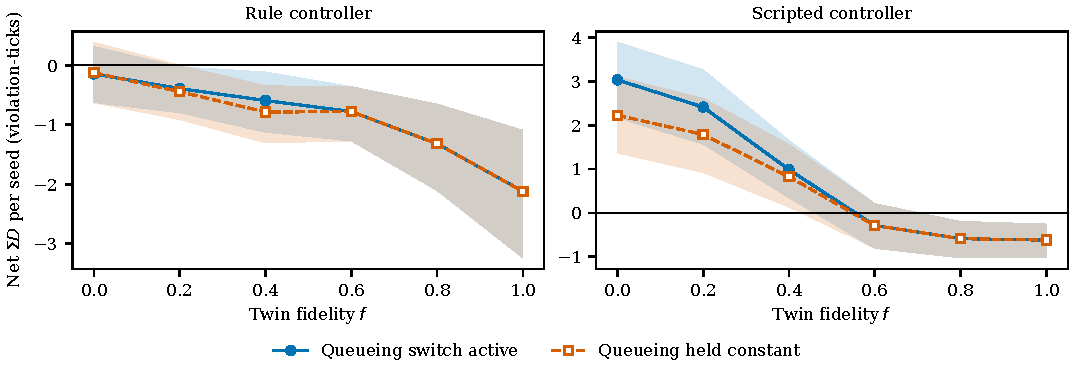
\includegraphics[width=\textwidth]{fig1_net_sum_d}
\caption{\NetSD{} per seed over approved candidates against twin fidelity, $n=150$ seeds. Shaded bands are 95\% seed-bootstrap intervals; solid circles: queueing switch active; dashed squares: queueing held constant. Negative values mean the approved set is locally better than reject-all. Scripted crossing: 0.555 [0.471, 0.677] (switch active), 0.549 [0.434, 0.677] (held constant).}
\label{fig:netsd}
\end{figure*}
For the scripted controller, \netSD{} falls monotonically from \ensuremath{+}3.033 at $f=0$ to \ensuremath{-}0.620 at $f=1$ and crosses zero at 0.555 [0.471, 0.677] (Fig.~\ref{fig:netsd}). The crossing lies between $f=0.4$ and $f=0.6$, exactly where the queueing switch flips, so as first observed it could not be attributed to fidelity. It became attributable only after the control that holds the queueing model constant: the crossing then sits at 0.549 [0.434, 0.677], monotone, with 4{,}997 of 5{,}000 resamples showing exactly one crossing. The 0.4$\rightarrow$0.6 step in the held-constant condition is \ensuremath{-}1.113 [\ensuremath{-}1.753, \ensuremath{-}0.507], while the switch itself is worth only \ensuremath{-}0.160 [\ensuremath{-}0.813, \ensuremath{+}0.480] per seed at $f=0.4$ ($p=0.61$). The rule controller's \netSD{} is at or below zero at every level in both conditions (\ensuremath{-}0.147 to \ensuremath{-}2.120), with no crossing; held constant, its curve is flat between 0.4 and 0.6 (\ensuremath{+}0.007 [\ensuremath{-}0.133, \ensuremath{+}0.193]) and is not fitted through.

\subsection{Episode-Level Benefit for the Rule Controller}
\begin{figure}[t]
\centering
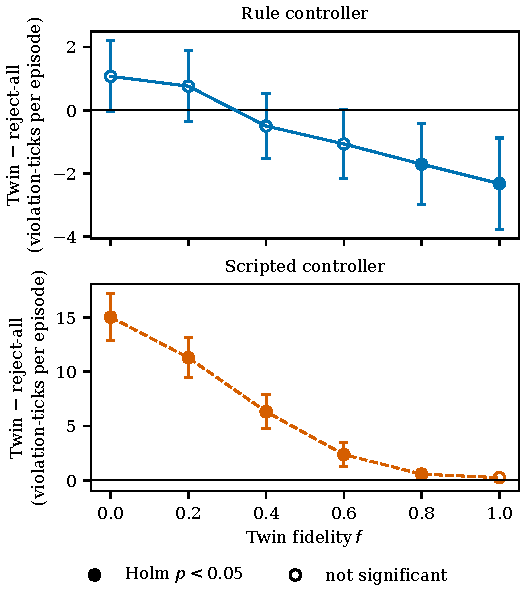
\includegraphics[width=\columnwidth]{fig2_episode_difference}
\caption{Episode-level difference, twin $-$ reject-all, by fidelity (condition (i), $n=150$). Bars are 95\% $t$-intervals; filled markers: Holm $p<0.05$; open markers: not significant. Negative means the twin gate is better.}
\label{fig:episode}
\end{figure}
Only for the rule controller does the twin beat reject-all at the episode level: by \ensuremath{-}2.320 [\ensuremath{-}3.762, \ensuremath{-}0.878] at fidelity 1.0 (exact Wilcoxon $p=\ensuremath{9.7\times 10^{-4}}$, Holm $p=0.0078$) and \ensuremath{-}1.707 [\ensuremath{-}2.987, \ensuremath{-}0.426] at 0.8 (Holm $p=0.025$), identically in both queueing conditions. The effect is small: about 1.9\% of the 122.1-tick reject-all baseline. It is concentrated in 22 of 150 seeds (14.7\%), and 4 of those seeds went the wrong way (18 better). The fidelity-1.0 result survives Bonferroni correction across the 30 unique comparisons of both controllers and both conditions (adjusted $p=0.029$); the fidelity-0.8 result does not (adjusted $p=0.107$). An earlier 10-seed estimate for this comparison overstated the effect and is superseded by the 150-seed values reported here. For the scripted controller, twin@1.0 is not distinguishable from reject-all (\ensuremath{+}0.233 [\ensuremath{-}0.156, \ensuremath{+}0.622], $p=0.287$, observed power 0.21).

\subsection{Classifier Quality}
\begin{table}[t]
\centering
\caption{Twin@1.0 as a classifier of harmful actions ($D>\theta$). Scripted: 1{,}167 candidates (29 beneficial); rule: 159 (30 beneficial). False positives split into definitional ($\tau<D\le\theta$) and predictive.}
\label{tab:classifier}
\footnotesize
\setlength{\tabcolsep}{2.5pt}
\begin{tabular}{@{}lcrrrrr@{}}
\toprule
Ctrl. & ($\tau,\theta$) & Recall & FPR & Neg. & FP def. & FP pred. \\
\midrule
Scr. & (0,3) & 0.996 & 0.256 & 262 & 56 & 11 \\
Scr. & (1,1) & 0.990 & 0.062 & 209 & 0 & 13 \\
Scr. & (3,3) & 0.996 & 0.065 & 262 & 0 & 17 \\
Rule & (0,3) & 0.989 & 0.075 & 67 & 3 & 2 \\
Rule & (1,1) & 0.979 & 0.047 & 64 & 0 & 3 \\
Rule & (3,3) & 0.989 & 0.060 & 67 & 0 & 4 \\
\bottomrule
\end{tabular}
\end{table}
\begin{figure}[t]
\centering
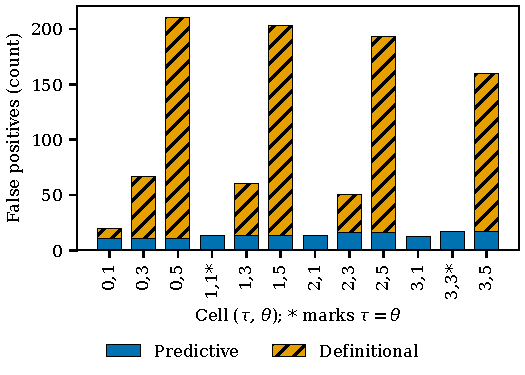
\includegraphics[width=\columnwidth]{fig4_false_positives}
\caption{False positives of the scripted controller's twin@1.0 across ($\tau,\theta$) cells, split into definitional ($\tau<D\le\theta$) and predictive. The definitional band is empty on the $\tau=\theta$ diagonal (marked *).}
\label{fig:fp}
\end{figure}
\textbf{(a) Reading the classifier on the $\tau=\theta$ diagonal.} At the operating setting $\tau=0$, $\theta=3$, the scripted twin@1.0 has FPR 0.256 [0.196, 0.323], but 56 of its 67 false positives (83.6\%) are definitional: actions with $0<D\le3$ that cause real harm below $\theta$. On the diagonal that band is empty by construction, so every false positive is a genuine prediction error. At $\tau=\theta=3$ recall is 0.996 and FPR is 0.065 [0.032, 0.105] (Table~\ref{tab:classifier}, Fig.~\ref{fig:fp}); the rule twin gives FPR 0.047--0.060 with recall 0.979--0.989. These rates rest on few negatives (262 scripted, 67 rule) and, for the rule controller, on 159 candidates in total; they describe a good filter on these candidates, not a general classifier.

\textbf{(b) The operating point.} The diagonal is where the classifier is read, not where the gate should run. At $\tau=3$ the scripted gate's \netSD{} turns positive, \ensuremath{+}0.173 [\ensuremath{-}0.340, \ensuremath{+}0.600], against \ensuremath{-}0.620 [\ensuremath{-}1.047, \ensuremath{-}0.267] at $\tau=0$, because a tolerance of 3 admits harmful scale-ups. The $\tau>0$ rows relabel a fixed corpus of decisions taken at $\tau=0$; they do not simulate a system running at $\tau>0$.

\subsection{The Benefit Ceiling}
\begin{figure}[t]
\centering
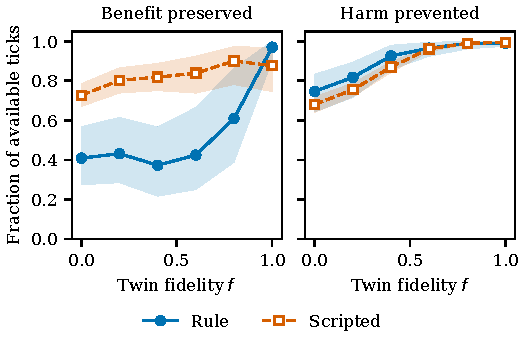
\includegraphics[width=\columnwidth]{fig3_benefit_harm}
\caption{Benefit preserved and harm prevented against twin fidelity (condition (i), $n=150$), with 95\% seed-bootstrap intervals.}
\label{fig:bphp}
\end{figure}
A gate cannot beat reject-all by more than the benefit reject-all discards. On the reject-all trajectory that benefit is 439 violation-ticks (2.93 per seed) in 23 of 150 seeds for the rule controller, and 52 ticks (0.35 per seed) in 12 seeds for the scripted controller, whose reject-all trajectory holds 15 beneficial against 922 harmful scale-ups. Seeds with a beneficial candidate in any arm number 59 (rule) and 149 (scripted), but most of that benefit exists only on trajectories that earlier actions created. Harm prevented rises with fidelity for both controllers; benefit preserved for the rule controller is flat up to 0.6 and rises only at 0.8--1.0 (Fig.~\ref{fig:bphp}). The scripted null at fidelity 1.0 is therefore structural.

\subsection{Live-Model Descriptive Study}
\begin{figure}[t]
\centering
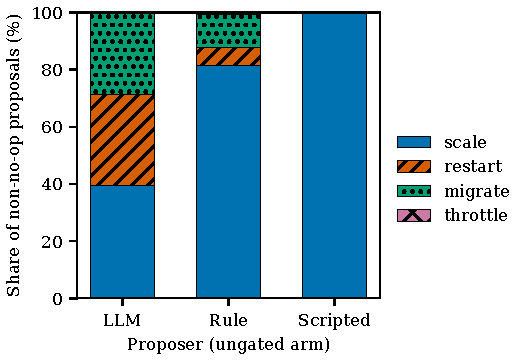
\includegraphics[width=\columnwidth]{fig5_action_mix}
\caption{Action-type mix of non-no-op proposals on the ungated arm: live model (30 seeds), rule and scripted controllers (150 seeds).}
\label{fig:mix}
\end{figure}
\begin{figure}[t]
\centering
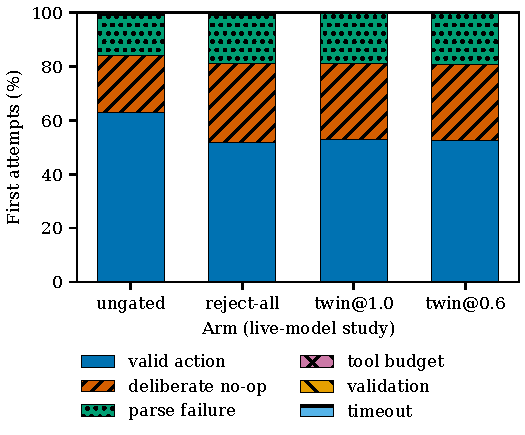
\includegraphics[width=\columnwidth]{fig6_llm_outcomes}
\caption{Live-model first-attempt outcome at each scheduled decision, by arm (30 seeds, 360 first attempts per arm).}
\label{fig:outcomes}
\end{figure}
A hosted model (gemini-3.6-flash, temperature 0.0, one prompt) was run as a proposer on 30 seeds with ungated, reject-all, twin@1.0 and twin@0.6 arms. This study is descriptive. Valid non-no-op first proposals occurred at 51.9\%--63.1\% of scheduled decisions, and final parse failures at 14.7\%--19.2\%, each resolved to an explicit no-op fallback (Fig.~\ref{fig:outcomes}). The model's action mix differs from both baselines: on the ungated arm 39.6\% scale, 31.7\% restart and 28.6\% migrate, against 81.4\% scale for the rule controller and 100.0\% for the scripted one (Fig.~\ref{fig:mix}). Recoverable benefit on the reject-all trajectory is 252 ticks, 8.40 per seed in 12 of 30 seeds, larger per seed than for either baseline. The paired twin@1.0 $-$ reject-all difference, \ensuremath{-}4.300 [\ensuremath{-}9.159, \ensuremath{+}0.559] (exact Wilcoxon $p=0.055$, Holm $p=0.109$, observed power 0.48), is an underpowered pilot statistic; no episode-level effect is claimed.

\subsection{Expected Versus Actual: Local Counterfactuals Do Not Compose}
\begin{table}[t]
\centering
\caption{Expected advantage (\netSD{}, Eq.~\eqref{eq:expadv}) versus actual episode difference against reject-all, per seed, condition (i), $n=150$.}
\label{tab:expected}
\footnotesize
\setlength{\tabcolsep}{4pt}
\begin{tabular}{@{}lrrrr@{}}
\toprule
& \multicolumn{2}{c}{Rule} & \multicolumn{2}{c}{Scripted} \\
\cmidrule(lr){2-3}\cmidrule(lr){4-5}
Fidelity & Expected & Actual & Expected & Actual \\
\midrule
0.0 & \ensuremath{-}0.147 & \ensuremath{+}1.073 & \ensuremath{+}3.033 & \ensuremath{+}15.013 \\
0.2 & \ensuremath{-}0.393 & \ensuremath{+}0.760 & \ensuremath{+}2.413 & \ensuremath{+}11.280 \\
0.4 & \ensuremath{-}0.593 & \ensuremath{-}0.500 & \ensuremath{+}0.987 & \ensuremath{+}6.313 \\
0.6 & \ensuremath{-}0.780 & \ensuremath{-}1.067 & \ensuremath{-}0.287 & \ensuremath{+}2.367 \\
0.8 & \ensuremath{-}1.320 & \ensuremath{-}1.707 & \ensuremath{-}0.587 & \ensuremath{+}0.560 \\
1.0 & \ensuremath{-}2.120 & \ensuremath{-}2.320 & \ensuremath{-}0.620 & \ensuremath{+}0.233 \\
\bottomrule
\end{tabular}
\end{table}
\NetSD{} is a sum of 20-tick counterfactuals with a no-op continuation, and it does not add up to closed-loop episode effects (Table~\ref{tab:expected}). For the scripted controller at fidelity 1.0, \netSD{} is \ensuremath{-}0.620 per seed, predicting a twin advantage, while the episode difference is \ensuremath{+}0.233: the sign is wrong. The scripted \netSD{} crossing near 0.555 has no episode-level counterpart; the episode curve approaches zero from above and never crosses. The mechanism is visible in single seeds of the earlier 10-seed ablation runs, cited as worked examples and not as effect estimates: on seed 2, approved scale-ups summed to \ensuremath{-}13 locally, but the episode ended \ensuremath{+}5 ticks worse than reject-all, because approved scale-ups alter later states that the no-op continuation does not represent. For the rule controller the sign is right but migrations are underestimated: on seed 65 of the gateway-exposed ablation the observed episode effect was 3.3$\times$ the local sum with the gateway immune (\ensuremath{-}7 predicted, \ensuremath{-}23 observed) and 6.0$\times$ with the gateway faultable (\ensuremath{-}8 predicted, \ensuremath{-}48 observed), because a migration's downtime is paid inside the horizon while its benefit accrues for the rest of the fault. Local metrics describe the filter; performance claims need episode outcomes.

\section{Limitations and Future Work}
\label{sec:limits}

\textbf{Shared simulator code.} The twin and the labeller are forks of the same simulator, so model-structure error is represented only through the five degradation axes; fidelity 1.0 is a harness sanity check, not an attainable twin.

\textbf{Relabelled corpus.} The $\tau>0$ rows of the classifier analysis relabel decisions taken at $\tau=0$; they are not simulations of a gate running at $\tau>0$.

\textbf{Shared response cache in the live study.} One response cache served all arms of the live-model study, so arms reuse identical responses for identical prompts, and which arm first queries the model depends on execution order.

\textbf{Synthetic-only evaluation.} All results come from a synthetic simulator with a gateway that is immune to node faults in the primary protocol. No numerical comparison with systems evaluated on realistic replicas, such as Aether~\cite{aether}, is meaningful.

\textbf{Incomplete cost accounting.} The historical live study retained input and visible-output tokens but not thinking tokens or failed-request usage; its rate-card figure (\$10.53 for 5{,}644 billed calls) is not an invoice.

\textbf{Future work.} The live-model evidence is a single model, prompt and cache realisation at 30 seeds. The normal-approximation requirement computed from the 30-seed data is $n=72$ seeds for 80\% power on the twin@1.0 $-$ reject-all comparison, and a 72-seed live-model confirmation run is scheduled. A workload with more restart and migration opportunities per episode would raise the benefit ceiling more efficiently than more seeds, and fault-arrival uncertainty could be modelled with legitimately available information such as disturbance ensembles~\cite{ddsafety,pomdpsurvey}.

\section{Conclusion}
Comparing a twin gate with reject-all on counterfactually labelled proposals separates what the twin predicts from what it blocks. On 150 seeds the twin's value depends strongly on fidelity: low fidelity is worse than no gate, and the net local benefit crosses zero near 0.549 once the queueing model is held constant. The episode-level gain is real for one controller, small, concentrated in a few seeds and bounded by the benefit reject-all discards. Classifier quality should be read on the $\tau=\theta$ diagonal, and local counterfactual metrics describe the filter but do not compose into episode effects.

\section*{Funding Statement}
The authors declare that no funding, grants, or external support were received during the development of this work.

\section*{Declaration of Competing Interest}
The authors declare that they have no known competing financial interests or personal relationships that could have appeared to influence the work reported in this paper.

\section*{Data Availability}
All data are generated by the simulator and are reproducible from the seeds reported here. The source code, experiment scripts and machine-readable results (\texttt{docs/research/extended\_fidelity\_sweep.json} and \texttt{docs/research/llm\_descriptive\_study.json}) are available at \url{https://github.com/NitinTheGreat/twin-in-the-loop}.

\begin{thebibliography}{99}

\bibitem{microremed} ``MicroRemed: Benchmarking LLMs in microservices remediation,'' arXiv:2511.01166, 2025.

\bibitem{nika} ``A network arena for benchmarking AI agents on network troubleshooting,'' arXiv:2512.16381, 2025.

\bibitem{netagentbench} ``NetAgentBench: A state-centric benchmark for evaluating agentic network configuration,'' arXiv:2604.09678, 2026.

\bibitem{aether} ``Aether: Network validation using agentic AI and digital twin,'' arXiv:2604.18233, 2026.

\bibitem{processplant} ``Leveraging LLM agents and digital twins for fault handling in process plants,'' in \emph{Proc. IEEE Int. Conf. Emerging Technologies and Factory Automation (ETFA)}, 2025, arXiv:2505.02076.

\bibitem{twingatedorch} ``Digital-twin validation gate between an optimisation agent and the execution layer in infrastructure orchestration,'' arXiv:2602.10900 and arXiv:2604.09705, 2026 (bibliographic details to be verified).

\bibitem{bbsimplex} U.~Mehmood, S.~Sheikhi, S.~Bak, S.~A. Smolka, and S.~D. Stoller, ``The Black-Box Simplex architecture for runtime assurance of autonomous CPS,'' in \emph{Proc. NASA Formal Methods Symp. (NFM)}, LNCS vol.~13260. Cham, Switzerland: Springer, 2022, doi:10.1007/978-3-031-06773-0\_12.

\bibitem{wabersich} K.~P. Wabersich and M.~N. Zeilinger, ``A predictive safety filter for learning-based control of constrained nonlinear dynamical systems,'' \emph{Automatica}, vol.~129, 109597, 2021, doi:10.1016/j.automatica.2021.109597.

\bibitem{dmps} A.~Banerjee, K.~Rahmani, J.~Biswas, and I.~Dillig, ``Dynamic model predictive shielding for provably safe reinforcement learning,'' in \emph{Proc. NeurIPS}, 2024.

\bibitem{mpcreview} M.~Schwenzer, M.~Ay, T.~Bergs, and D.~Abel, ``Review on model predictive control: An engineering perspective,'' \emph{Int. J. Adv. Manuf. Technol.}, vol.~117, pp.~1327--1349, 2021, doi:10.1007/s00170-021-07682-3.

\bibitem{netinjectbench} ``NetInjectBench: Benchmarking indirect prompt injection in tool-using large language model agents for network operations,'' arXiv:2607.10490, 2026.

\bibitem{agentdojo} E.~Debenedetti, J.~Zhang, M.~Balunovi\'c, L.~Beurer-Kellner, M.~Fischer, and F.~Tram\`er, ``AgentDojo: A dynamic environment to evaluate prompt injection attacks and defenses for LLM agents,'' in \emph{Proc. NeurIPS Datasets and Benchmarks Track}, 2024.

\bibitem{fidelityam} C.~Su, B.~Hicks, and A.~Nassehi, ``Investigating the influence of fidelity on the capability of a digital twin to detect material extrusion failures,'' \emph{Journal of Intelligent Manufacturing}, vol.~35, pp.~2263--2276, 2024, doi:10.1007/s10845-023-02144-x.

\bibitem{mbrlsurvey} F.-M. Luo, T.~Xu, H.~Lai, X.-H. Chen, W.~Zhang, and Y.~Yu, ``A survey on model-based reinforcement learning,'' \emph{Science China Information Sciences}, vol.~67, 121101, 2024, doi:10.1007/s11432-022-3696-5.

\bibitem{robustdiag} L.~K. Carvalho, M.~V. Moreira, and J.~C. Basilio, ``Comparative analysis of related notions of robust diagnosability of discrete-event systems,'' \emph{Annual Reviews in Control}, vol.~51, pp.~23--36, 2021.

\bibitem{pomdpsurvey} M.~Lauri, D.~Hsu, and J.~Pajarinen, ``Partially observable Markov decision processes in robotics: A survey,'' \emph{IEEE Trans. Robot.}, vol.~39, no.~1, pp.~21--40, 2023, doi:10.1109/TRO.2022.3200138.

\bibitem{k8scontroller} The Kubernetes Authors, ``Controllers,'' Kubernetes documentation. Accessed: Sep.~23, 2026. [Online]. Available: \url{https://kubernetes.io/docs/concepts/architecture/controller/}

\bibitem{k8shpa} The Kubernetes Authors, ``Horizontal Pod Autoscaling,'' Kubernetes documentation. Accessed: Sep.~23, 2026. [Online]. Available: \url{https://kubernetes.io/docs/concepts/workloads/autoscaling/horizontal-pod-autoscale/}

\bibitem{metastable} L.~Huang, M.~Magnusson, A.~B. Muralikrishna, S.~Estyak, R.~Isaacs, A.~Aghayev, T.~Zhu, and A.~Charapko, ``Metastable failures in the wild,'' in \emph{Proc. USENIX Symp. Operating Systems Design and Implementation (OSDI)}, 2022.

\bibitem{budgetaware} Liu \emph{et al.}, ``Budget-aware tool use enables effective agent scaling,'' arXiv:2511.17006, 2025.

\bibitem{langgraph} LangChain, ``Graph API: Recursion limit,'' LangGraph documentation. Accessed: Sep.~23, 2026. [Online]. Available: \url{https://docs.langchain.com/oss/python/langgraph/graph-api}

\bibitem{stochsim} B.~L. Nelson and L.~Pei, \emph{Foundations and Methods of Stochastic Simulation: A First Course}, 2nd ed. Cham, Switzerland: Springer, 2021, doi:10.1007/978-3-030-86194-0.

\bibitem{yadav} Yadav \emph{et al.}, ``Using common random numbers for simulation-based planning with rollouts,'' in \emph{Proc. Reinforcement Learning Conference (RLC)}, 2026.

\bibitem{rulebasedshield} Shperberg \emph{et al.}, ``A rule-based shield: Accumulating safety rules from catastrophic action effects,'' in \emph{Proc. Conference on Lifelong Learning Agents (CoLLAs)}, PMLR vol.~199, 2022.

\bibitem{saferlsurvey} ``A survey of safe reinforcement learning and constrained MDPs: A technical survey on single-agent and multi-agent safety,'' arXiv:2505.17342, 2025.

\bibitem{slbench} ``SLBench,'' arXiv:2607.09016, 2026.

\bibitem{ddsafety} K.~P. Wabersich, A.~J. Taylor, J.~J. Choi, K.~Sreenath, C.~J. Tomlin, A.~D. Ames, and M.~N. Zeilinger, ``Data-driven safety filters: Hamilton--Jacobi reachability, control barrier functions, and predictive methods for uncertain systems,'' \emph{IEEE Control Systems Magazine}, vol.~43, no.~5, pp.~137--177, 2023.

\bibitem{vagram} C.~Voelcker, V.~Liao, A.~Garg, and A.-m. Farahmand, ``Value gradient weighted model-based reinforcement learning,'' in \emph{Proc. Int. Conf. Learning Representations (ICLR)}, 2022.

\bibitem{petridiag} Y.~Pencol\'e and A.~Subias, ``Diagnosability of event patterns in safe labeled time Petri nets: A model-checking approach,'' \emph{IEEE Trans. Autom. Sci. Eng.}, vol.~19, no.~2, pp.~1151--1162, 2022.

\bibitem{rcasurvey} J.~Soldani and A.~Brogi, ``Anomaly detection and failure root cause analysis in (micro)service-based cloud applications: A survey,'' \emph{ACM Computing Surveys}, vol.~55, no.~3, 2022, doi:10.1145/3501297.

\bibitem{mlstats} O.~Rainio, J.~Teuho, and R.~Kl\'en, ``Evaluation metrics and statistical tests for machine learning,'' \emph{Scientific Reports}, vol.~14, 6086, 2024, doi:10.1038/s41598-024-56706-x.

\bibitem{multtest} O.~Menyhart, B.~Weltz, and B.~Gy\H{o}rffy, ``MultipleTesting.com: A tool for life science researchers for multiple hypothesis testing correction,'' \emph{PLoS ONE}, vol.~16, no.~6, e0245824, 2021, doi:10.1371/journal.pone.0245824.

\bibitem{probcomputing} M.~Harchol-Balter, \emph{Introduction to Probability for Computing}. Cambridge, U.K.: Cambridge University Press, 2023.

\end{thebibliography}

\end{document}
